\documentclass[a4paper, 12pt]{scrartcl}
\usepackage[utf8]{inputenc}
\usepackage[ngerman]{babel}
\usepackage[T1]{fontenc}
\usepackage{graphicx}
\usepackage{hyperref}
\usepackage{array}
\usepackage{longtable}
\renewcommand{\arraystretch}{1.5} 
\hypersetup{
	colorlinks=true,
	linkcolor=blue,
	filecolor=blue,      
	urlcolor=blue,
	pdftitle={ Example},
	pdfpagemode=FullScreen,
}



\title{End-2-End-Prozess}
\titlehead{Praxisbericht}
\author{Maksym Mykhailych}
\date{09. September 2025}

\begin{document}
	\maketitle
	\newpage
	\section*{Abstract}
	\newpage 	
	\tableofcontents
	\newpage
	
	\newpage
	\section{Einleitung}
	Einleitender Text.
	\newpage
	\subsection{Motivation}
	\subsection{Aufgabenstellung}
	\subsection{Aufbau der Arbeit}
	Text.
	\newpage
	\section{Grundlagen}
	\subsection{Unternehmenseinführung in Capgemini} %VOrstellung von Capgemini(Geschichte, Zahlen, Wie groß?)
	Capgemini, mit Hauptsitz in Paris, ist ein transnationales, börsennotiertes Unternehmen, das Beratungs-, Technologiedienstleistungen und digitale Transformationslösungen anbietet. Das Unternehmen bietet eine Vielzahl von Dienstleistungen, darunter Beratung, Technologie. Mit einer Präsenz in über 50 Ländern bedient Capgemini Kunden aus diversen Branchen, einschließlich Finanzdienstleistungen, Automobilindustrie, Gesundheitswesen und Einzelhandel etc. Im Jahr 2023(Abb. \ref{Stand von Capgemini}) erzielte Capgemini einen Umsatz von 22,5 Milliarden Euro und beschäftigt weltweit etwa 340.000 Mitarbeiter.!!!!
	\begin{figure}[h!]
		\begin{center}
			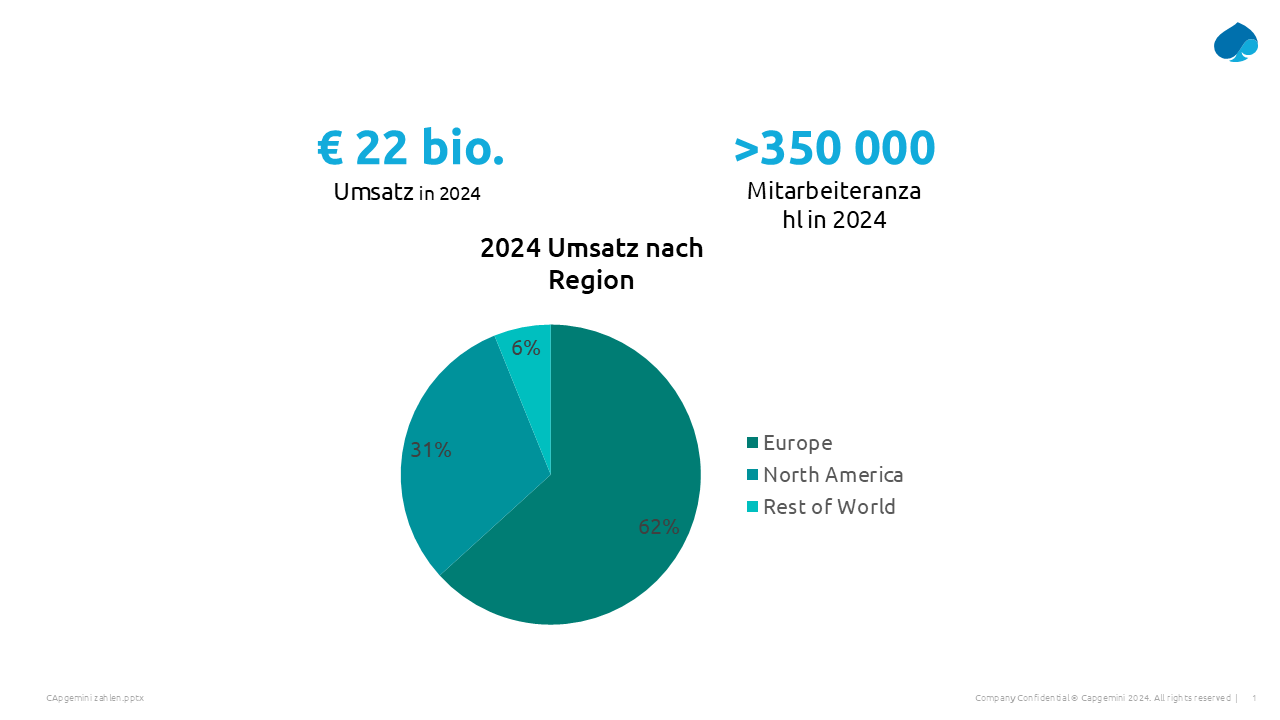
\includegraphics[width=8cm]{CApgemini zahlen.png}
			\caption{Jahresbericht von Capgemini in 2024\cite{Capgemini_allgemein}}
			\label{Stand von Capgemini}
		\end{center}
	\end{figure}
	\subsubsection{Struktur und Organisation in Deutschland}
	
	Capgemini Gruppe bietet ihren Kunden eine End-to-End-IT-Transformation, die von der Umgestaltung komplexer IT-Architekturen bis hin zur Entwicklung spezifischer kleiner Funktionen reicht. In diesem Zusammenhang verfügt Capgemini über große Mitarbeiteranzahl und besteht aus mehreren Marken:
	\begin{itemize}
		\item \textbf{Capgemini Invent\cite{Capgemini_invent}:} Diese Sparte konzentriert sich auf die strategische digitale Entwicklung der Kunden.
		\item \textbf{Capgemini\cite{Capgemini}:} Das Mutterunternehmen bietet ein breites Spektrum an Dienstleistungen, darunter IT-Beratung und Technologie-Services.
		\item \textbf{Capgemini Engineering\cite{Capgemini_eng}:} Ein weltweit führender Anbieter von Engineering- und F\&E-Dienstleistungen, der Kunden dabei unterstützt, ihren Weg zur Intelligent Industry zu beschleunigen.
		\item \textbf{Sogeti\cite{Sogeti}:} Entwickelt, testet und schützt innovative Anwendungen für Unternehmen und stützt sich dabei auf Expertise in den Bereichen Beratung, Testen, agile und Cloud-Entwicklung sowie Cybersicherheit.
	\end{itemize}
	Dies sind die wichtigsten Marken von Capgemini in Deutschland. Meine Erfahrung habe ich im Mutterunternehmen von Capgemini gesammelt, wo das Unternehmen auch intern in verschiedene Abteilungen unterteilt ist. Meine Tätigkeit fand in der Abteilung statt, die paketbasierte Lösungen %Im glossar erklären was PBS ist(SAP, Windchill etc.)
	für Kunden anbietet.
	
	
	\subsection{Definition des End-2-End-Prozesses}
	Ein End-to-End-Prozess(End-2-End) bezeichnet den Ablauf einer Aktion vom Anfang bis zum logischen Ende. Es gibt verschiedene End-to-End-Prozesse, die in Unternehmen betrachtet werden können. Zum Beispiel ist im Bereich Human Resources der sogenannte Hire-to-Retire-Prozess relevant, in der Logistik der Supply-Chain-Prozess und im Bereich des Product Lifecycle Management (PLM) der End-to-End-Prozess des Produktlebenszyklus.
	\subsubsection{Überblick des allgemeinen End-2-End-Prozesses} %wie sieht algemein E2E-Prozess bei der Beratung!
	%Wie bei allen Unternehmen ist die Hauptaufgabe der Consultingsunternehmen, den eigenen Unsatz und das Gewinn jährlich zu steigern. 
	In dieser Arbeit wird der gesamte Prozess des Projektmanagements betrachtet. Das Projektmanagement besteht üblicherweise aus fünf auf Abbildung \ref{Projektmanagment} gezeigten Phasen\cite{timinger2024modernes}
	\begin{figure}[h!]
		\begin{center}
			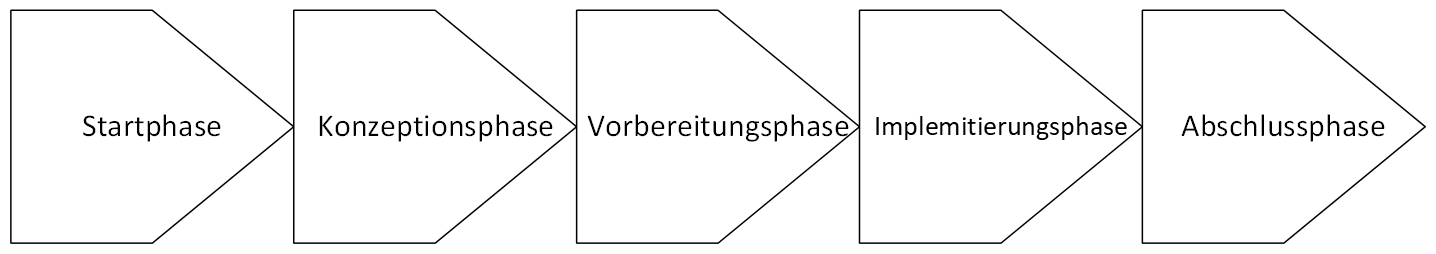
\includegraphics[width=12cm]{Drawing.png}
			\caption{Phasenplan\cite{timinger2024modernes}}
			\label{Projektmanagment}
		\end{center}
		
	\end{figure}
	\begin{enumerate}
		\item \textbf{Startphase:} 
		In dieser Phase erfolgt die Initiierung des Projekts, wobei die grundlegenden Ziele und Anforderungen, Nachfrage definiert werden. Die strategische Ausrichtung des Projekts wird durch die Fachbereichsleiter sowie die Stakeholder festgelegt.
		\item \textbf{Konzeptionsphase:}
		Auf Grundlage der definierten Ziele entwickeln die Fachbereichsleiter (z. B. die Leiter der Abteilungen IT, Ressourcenmanagement und HR) detaillierte Pläne und Konzepte zur Umsetzung des Projekts. In diesem Rahmen wird bestimmt, welche Mitarbeiter und Materialien erforderlich sind. Zudem wird überprüft, ob das Unternehmen über die benötigten Fachkräfte verfügt oder ob eine externe Rekrutierung notwendig ist.
		\item \textbf{Vorbereitungsphase:} 
		In dieser Phase werden die für die Projektdurchführung erforderlichen Ressourcen und Materialien beschafft sowie die organisatorischen Strukturen eingerichtet. Dabei übernehmen insbesondere der Projektleiter, das Beschaffungsteam und die Fachbereichsleiter eine zentrale Rolle, indem sie sicherstellen, dass alle notwendigen Ressourcen bereitgestellt werden.
		\item \textbf{Implementierungsphase:}  
		Die Umsetzung des Projekts erfolgt gemäß den zuvor entwickelten Plänen und Konzepten. Während dieser Phase überwachen der Projektleiter, das Projektteam und die Qualitätssicherung den Fortschritt, um die termingerechte und qualitativ hochwertige Durchführung der Maßnahmen sicherzustellen.
		\item \textbf{Abschlussphase:} 
		Nach der Umsetzung wird das Projekt formal abgeschlossen. Dabei erfolgt eine Bewertung der Ergebnisse, und die Projektdokumentation wird erstellt. Zudem wird ein Plan zur Vermarktung des Produkts entwickelt, um eine effiziente Markteinführung und einen erfolgreichen Vertrieb sicherzustellen. Der Projektleiter, das Projektteam sowie die Stakeholder sind maßgeblich an der Evaluierung der Projektergebnisse, der Erstellung der Dokumentation und der Entwicklung der Verkaufsstrategie beteiligt.
		%REFERENZIEREN
	\end{enumerate}
	Jedes Projekt unterscheidet sich in Zielen, Inhalten und Dauer. Dennoch ist der Projektablauf meist ähnlich strukturiert. Typischerweise umfasst er die folgenden Phasen: Initiierung, Planung, Durchführung, Überwachung und Abschluss. Diese allgemeinen Phasen ermöglichen eine systematische und effiziente Projektabwicklung, unabhängig von den spezifischen Unterschieden zwischen den Projekten\cite{wegmann2006projektmanagement}.
	\subsubsection{End-2-End-Prozess bei Capgemini}
	Capgemini ist zwar ein Beratungsunternehmen, das keine eigenen Produkte entwickelt, sondern andere Unternehmen unterstützt. Aus diesem Grund unterscheidet sich das Projektmanagement und die Projektphasen von denen in Industrieunternehmen. In Abbildung \ref{Projektmanagment_Campgeini} sind die folgenden 6 Projektphasen definiert \cite{wegmann2006projektmanagement}:
	\begin{figure}[h!]
		\begin{center}
			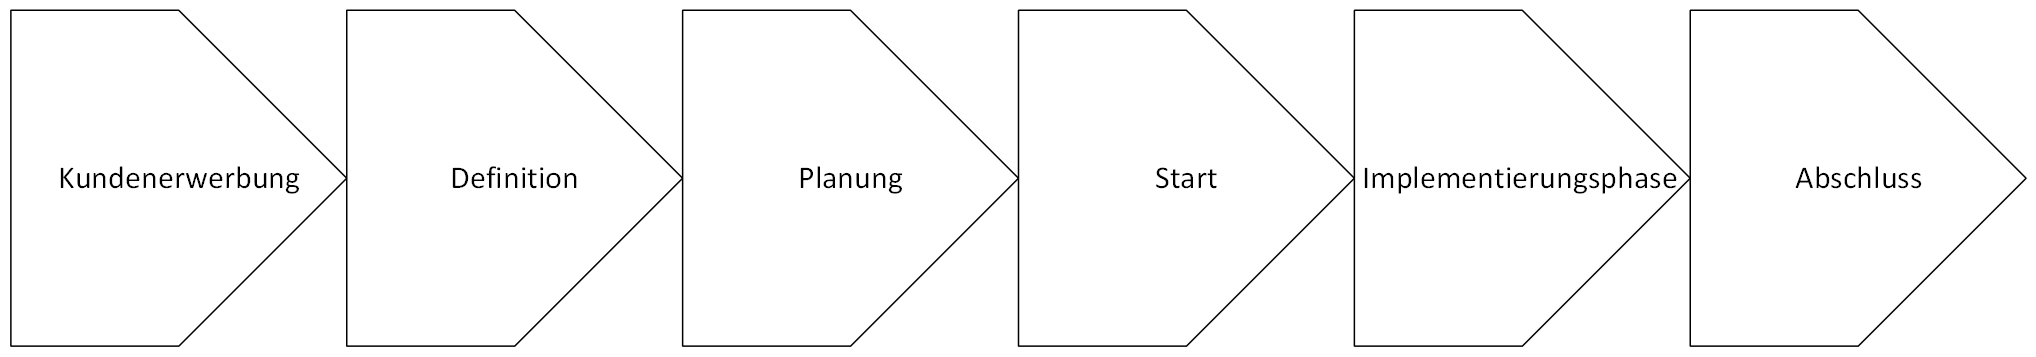
\includegraphics[width=12cm]{Projektmanagement_Capgemini .png}
			\caption{Phasenplan bei der Beratungsunternehmen \cite{wegmann2006projektmanagement}}
			\label{Projektmanagment_Campgeini}
		\end{center}
	\end{figure}
	\begin{enumerate}
		\item \textbf{Kundengewinnung:} In dieser Phase bemüht sich die Vertriebsabteilung von 		Capgemini, neue Projekte zu akquirieren. Dabei werden verschiedene Strategien eingesetzt, wie die Demonstration der Fachkompetenz von Capgemini in relevanten Bereichen, die Hervorhebung erfolgreicher Referenzprojekte und die Präsentation von Innovationen auf Messen. Zusätzlich werden potenzielle Kunden durch gezielte Marketingmaßnahmen und persönliche Kontakte angesprochen, um das Vertrauen in die Fähigkeiten von Capgemini zu stärken.
		\item \textbf{Definition:} In dieser Phase versucht Capgemini, den Bedarf des
		Unternehmens zu definieren. Außerdem wird der Vertrag diskutiert und ausgearbeitet, um die Rahmenbedingungen und Erwartungen klar festzulegen.
		
		\item \textbf{Planung:} In dieser Phase wird das Projekt detailliert geplant. Es wird 
		festgelegt, wie viel Zeit für die Durchführung des Projekts benötigt wird und welche Rollen und Ressourcen erforderlich sind. Das Staffing-Team wählt entsprechend qualifizierte Mitarbeiter aus, um die Projektanforderungen zu erfüllen.
		\item \textbf{Start:} In dieser Phase versucht das gebildete Team, das Problem zu definieren und eine ausführliche Lösung zu erarbeiten. Dies umfasst die Erstellung eines detaillierten Zeitplans sowie die Festlegung der Verantwortlichkeiten für die einzelnen Aufgaben.
		\item \textbf{Implementierungsphase:} Dies ist die zeitlich umfangreichste Phase, in der alle Pläne in die Realität umgesetzt werden. Jeder Mitarbeiter führt seine spezifischen Aufgaben aus, um die Projektziele zu erreichen.
		\item \textbf{Abschluss} Auch als sogenannte Abschlussphase bekannt, in der alle organisatorischen und finanziellen Fragen zwischen dem Unternehmen und Capgemini geklärt werden.
	\end{enumerate}
	\subsection{PLM-Systeme}
	Das Auto ist heutzutage ein unverzichtbarer Begleiter des Menschen, der ihn bei der schnellen Fortbewegung unterstützt. Aus der Sicht eines Ingenieurs jedoch ist es auch eine komplexe Maschine, die aus Hunderttausenden von Einzelteilen besteht, die effizient verwaltet werden müssen. In diesem Zusammenhang entstand zu Beginn des 21. Jahrhunderts ein neues Paradigma in Fertigungsunternehmen: das Product Lifecycle Management (PLM). PLM ermöglicht es Unternehmen, ihre Produkte während des gesamten Lebenszyklus zu überwachen und zu steuern. Das ist eine der wichtigsten Aktivitäten der Fertigungsunternehmen\cite{stark2011product}.
	\subsubsection{Allgemeine Übersicht der PLM-Systeme}
	Product Lifecycle Management (PLM) bezeichnet die Verwaltung des gesamten Lebenszyklus eines Produkts – von der Idee und Entwicklung über die Produktion und Nutzung bis hin zur Entsorgung oder zum Recycling. PLM kann sowohl ein einzelnes Produkt als auch das gesamte Produktportfolio eines Unternehmens verwalten\cite{stark2011product}.
	\newline
	Der Produktlebenszyklus kann aus mehreren Phasen bestehen, die jedoch in fünf Hauptphasen(Abb. \ref{PLM}) zusammengefasst werden können:
	\begin{figure}[h!]
		\begin{center}
			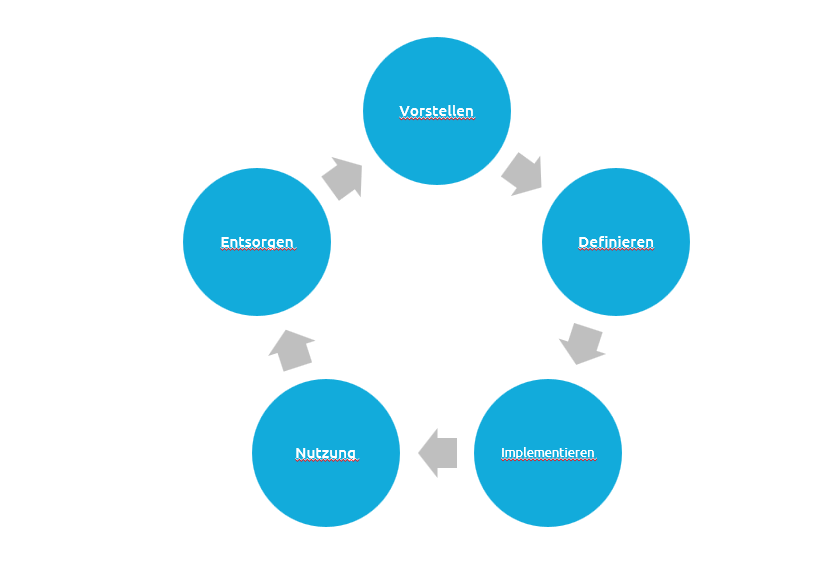
\includegraphics[width=12cm]{PLM.png}
			\caption{ Product Lifecycle Management\cite{stark2011product}}
			\label{PLM}
		\end{center}
	\end{figure}
	\begin{itemize}
		\item \textbf{Vorstellen:} In dieser Phase wird das Produkt geplant. Das Unternehmen analysiert die Marktbedingungen sowie die voraussichtlichen Kosten für die Entwicklung des Produkts.
		\item \textbf{Definieren:} Hier wird die Entstehung des Produkts ausführlich geplant. Es wird ein Design skizziert, die Materialien für die Produktion werden festgelegt und andere technische Spezifikationen werden definiert.
		\item \textbf{Implementieren:} In dieser Phase beginnt die eigentliche Produktion des Produkts. Prozesse wie Montage, Qualitätskontrolle und Lieferkettenmanagement werden eingeführt.
		\item \textbf{Nutzen:} Das Produkt wird auf dem Markt verkauft und von den Kunden genutzt. Während dieser Phase stehen Kundenzufriedenheit, Wartung, Updates und Weiterentwicklungen im Fokus. Unternehmen sammeln Kundenfeedback, analysieren Leistungsdaten und bieten Support- oder Garantieprogramme an. Produktverbesserungen oder neue Versionen können aus dieser Phase hervorgehen.
		\item \textbf{Entsorgen:} In dieser Phase wird das Produkt vom Markt genommen. Unternehmen entwickeln Strategien für Recycling bzw. umweltfreundliche Entsorgung.
	\end{itemize}
	\textbf{\textit{Ich möchte hier auch als ein Beispiel mit z.B. PLM von Iphone hinzufügen, was denkt ihr dazu?}}
	\newline 
	\newline
In einem Unternehmen liegt die Verantwortung für ein Produkt in den verschiedenen Phasen seines Lebenszyklus bei unterschiedlichen Abteilungen. Während in der frühen Phase des Produktlebenszyklus das Marketing eine zentrale Rolle spielt, übernimmt in der Entwicklungsphase primär die Konstruktions- und Ingenieurabteilung die Verantwortung. In späteren Phasen, insbesondere während der Nutzung des Produkts, sind der Kundenservice und die Wartungsabteilung maßgeblich involviert. Heutzutage kann die Produktion auch in verschiedenen Ländern stattfinden.\newline
Aus diesem Grund treten Unternehmen bei der Entwicklung des Produkts auf mehrere Probleme, wie den Verlust der Kontrolle, was zu einer sinkenden Qualität führen kann. Zudem gibt es möglicherweise keine Möglichkeiten, das Produkt an verschiedenen Standorten zu fertigen\cite{stark2011product}.\newline
Ein Product Lifecycle Management (PLM)-System kann diesen Herausforderungen entgegenwirken, indem es eine zentrale Plattform für die Verwaltung und den Austausch produktbezogener Daten bietet. Durch die Standardisierung von Prozessen und eine einheitliche Datenbasis ermöglicht PLM eine effizientere Zusammenarbeit zwischen den Fachabteilungen, verbessert die Nachverfolgbarkeit von Produktänderungen und unterstützt fundierte Entscheidungsprozesse über den gesamten Lebenszyklus hinweg\cite{ozturk2019product}.
	\subsubsection{Vorstellung von verschiedenen Vendoren}
Auf dem Markt existieren viele verschiedene PLM-Systeme, auch sogenannte PLM-Vendoren. Dies sind Unternehmen, die spezialisierte Softwarelösungen entwickeln, die auf unterschiedliche Branchen, Unternehmensgrößen und Anforderungen zugeschnitten sind. Sie bieten Product Data Management (PDM)-Software an, um technische produktbezogene Inhalte zu erfassen, zu pflegen und zu verwalten. Diese Inhalte definieren die Produktspezifikationen und -designs sowie die zulässigen Produktkonfigurationen\cite{PLM1}.
Im Jahr 2023 wuchs der globale Markt für Product Lifecycle Management und Engineering (PLM)-Software auf nahezu 28,4 Milliarden US-Dollar, was einem Wachstum von 9,6\% entspricht. Die zehn größten Anbieter hielten einen bedeutenden Marktanteil von 85,7\%, wobei Dassault Systèmes mit 17,1\% führend war.Hier sind die Top-10 PLM-Vendoren im Jahr 2023 auf dem Markt\cite{Top10PLMVendoren}:
	\begin{enumerate}
		\item \textbf{Dassault Systèmes} 
		\item \textbf{Autodesk}
		\item \textbf{Synopsys}
		\item \textbf{Siemens Digital Industries Software}
		\item \textbf{Cadence Design Systems}
		\item \textbf{PTC}
		\item \textbf{Hexagon}
		\item \textbf{ANSYS}
		\item \textbf{Altair}
		\item \textbf{Bentley Systems}
	\end{enumerate}
	Capgemini bietet die Implementierung von PLM-Systemen für ihre Kunden an und arbeitet dabei mit vier Anbietern zusammen: Dassault Systèmes, PTC, Siemens Digital Industries Software und Aras. Wie schon ertwäht, bieten diese Unternehmen zunächst zentrumbildende PDM-Softwarelösungen.
	\begin{itemize}
		\item \textbf{Dessault Systemes\cite{Dessault}:} Ein französisches Softwareunternehmen, das sich auf 3D-Design, Simulation und  (PLM) spezialisiert hat. Es wurde 1981 gegründet und ist bekannt für seine 3DEXPERIENCE-Plattform, die in verschiedenen Industrien wie Luft- und Raumfahrt, Automobil und Medizintechnik eingesetzt wird.
		\item \textbf{PTC(Parametric Technology Corporation)\cite{PTC}:} Ein US-amerikanisches Unternehmen mit Sitz in Boston, das 1985 gegründet wurde. PTC bietet Softwarelösungen für CAD (Creo), PLM(Windchill) und IoT (ThingWorx) an. Besonders stark ist PTC in der digitalen Transformation und der Integration von Augmented Reality (Vuforia) in industrielle Prozesse.
		\item \textbf{Siemens Digital Industries Software\cite{Siemens}:} Ein Tochterunternehmen von Siemens mit Sitz in Plano, Texas, das sich auf 3D- und 2D-PLM-Software spezialisiert hat.  Eine der wichtigsten PLM-Lösungen von Siemens ist Teamcenter, das als zentrale Plattform für Produktdaten- und Prozessmanagement fungiert.
		\item \textbf{Aras\cite{Aras}:} Ein amerikanischer Entwickler und Herausgeber von Produktentwicklungssoftware, insbesondere Aras Innovator. Das Produkt wird für PLM und andere Zwecke verwendet.
	\end{itemize}
	Capgemini bietet umfassende Beratungs- und Implementierungsdienste für spezifische PLM-Systeme an, die auf die individuellen Bedürfnisse und Anforderungen der Kunden zugeschnitten sind. 
	\newpage
	\section{Phase 1: Kundenerwerbung} 
Auf dem Markt existiert eine vielfältige Anzahl von IT-Beratungsunternehmen, die von kleinen Boutique-Firmen bis hin zu großen Unternehmen wie Capgemini reichen. Alle Anbieter verfolgen das Ziel, Kunden zu gewinnen, und nutzen dafür unterschiedliche Ansätze, beispielsweise attraktive Verträge mit geringen Kosten und minimalem Risiko für die Kunden oder herausragende Präsentationen ihrer Arbeit mithilfe von Demonstratoren\cite{muhonen2013qualification}.
	\subsection{Ausgangslage und Aufgabenstallung} %Ich beschäftige mich mit der Showcase für die Kunden um das Projekt zu kriegen.
Capgemini ist ein großes Unternehmen mit verschiedenen Einheiten, die, wie bereits beschrieben, teilweise ähnliche Tätigkeiten ausführen. Die zentrale Abteilung "Product Lifecycle Management/Digital Manufacturing" von Capgemini \cite{Capgemini} verfügt über einige PLM-Demonstratoren. Ähnliche Demonstratoren existieren jedoch auch in anderen Einheiten, über die die zentrale Abteilung nur begrenzt informiert ist.\newline
Das Ziel des Managements ist es, eine zentrale Übersicht über alle vorhandenen PLM-Demonstratoren zu erstellen, damit alle Mitarbeitenden darauf zugreifen können. Dies soll nicht nur die Transparenz innerhalb des Unternehmens erhöhen, sondern auch die Kommunikation und Zusammenarbeit zwischen den verschiedenen Einheiten stärken.
	\subsection{Anforderungen für die Erstellung der Demonstratorenübersicht} %welche versionen die Demonstratoren haben, Ziel des Demonstrators, Beschreibungen etc.
Capgemini Deutschland vefügt über eine Vielzahl von Demonstratoren. Es soll eine toolgestützte Wiki-Übersicht erstellt werden, die verschiedene Analysemöglichkeiten bietet, wie etwa die Sortierung und Filterung der PLM-Demonstratoren nach Kriterien wie Vendoren oder Versionen.
Zudem ist sicherzustellen, dass die Seite leicht auffindbar ist. Dafür sollte sie auf einer zentralen Plattform integriert werden, die allen Mitarbeitenden zugänglich ist und eine intuitive Navigation gewährleistet.
	\subsection{Tools-Analyse}%Welche Tools gibt und welche sind geeignet für meinen Demostrator(Beschränung von Unternehmen betrachten)
Es existiertz zahlreiche Tools, um eine solche Übersicht zu erstellen, darunter Wiki.js, Jira Confluence, Microsoft SharePoint, Zendesk, ClickUp und viele mehr. Allerdings verwendet Capgemini in der Regel die Produkte von Atlassian und Microsoft . Aus diesem Grund wird die Priorität auf Confluence\cite{Confluence} und SharePoint\cite{SharePoint} gelegt, um die Demonstratorenübersicht zu entwickeln. Beide Tools sind starke Tools mit verschiedenen zwar Focus.
\newpage
	\begin{longtable}{|p{4.5cm}|p{5.5cm}|p{5.5cm}|}
		\hline
		\textbf{Kriterium} & \textbf{Confluence} & \textbf{SharePoint} \\ \hline
		\textbf{Wiki-Funktionalität} & Entwickelt als kollaborative Plattform für Wissensmanagement und Dokumentation & Kann als Wiki verwendet werden, aber primär für Dokumentenmanagement konzipiert \\ \hline
		\textbf{Datenintegration} & Nahtlose Integration mit Jira und anderen Atlassian-Produkten sowie Microsoft-Teams & Enge Integration mit Microsoft-Produkten, wie Power BI, PowerPoint usw..\\ \hline
		\textbf{Benutztfreundlichkeit} & Intuitiv und flexibel, ideal für Teams, die Inhalte gemeinsam bearbeiten & Komplexere Einrichtung, erfordert mehr Anpassung für Wiki-Zwecke\\ \hline
		\textbf{Suchenfunktionen} &starke Suchfunktionen mit Tags und Kategorien & Gute Suchfunktionen, aber weniger intuitiv für Wiki-Inhalte. Möglichkeit leicht die Seite durch internes Internet finden  \\ \hline
		\textbf{Kollaboration} &Echtzeit-Bearbeitung von Seiten und Kommentaren & wenig dynamisch, eher wie "branching" in GitHub \\ \hline
		\caption{Vergleich zwischen Jira Confluence und Micorosoft SharePoint}
	\end{longtable}
Einerseits ist es von hoher Bedeutung, dass die geplante Seite über umfassende Analysemöglichkeiten verfügt, was durch den Einsatz von Confluence effizient umgesetzt werden kann. Andererseits ist die Auffindbarkeit der Seite ebenso entscheidend. Angesichts der bestehenden Infrastruktur bei Capgemini ist es naheliegend, zwei SharePoint-Plattformen miteinander zu verknüpfen, da dies technisch leicht umsetzbar ist. Danach kann die Seite mit der Übersicht schnell gefunden werden. Darüber hinaus bietet SharePoint eine enge Integration mit Microsoft-365-Diensten wie Power BI, wodurch ebenfalls erweiterte Analysemöglichkeiten sich schaffen lassen.
	\subsection{Erstellung der Demonstratorenübersicht}
Zunächst sollte eine zentrale Seite erstellt werden, die eine Einführung und Erklärung der Übersicht bereitstellt. Diese Seite dient als Einstiegspunkt und verweist auf die spezifischen Seiten der verschiedenen PLM-Vendoren mit ausführlichen Informationen über Demostratoren. Die ausführliche Information über jeden Demostrator besteht aus Abteilung, Kontaktpersonen, Fähigkeiten, Kompatibilität, zusätzliche Dokumentation usw.. Für die Umsetzung dieser strukturierten Informationsübersicht eignet sich das benutzerfreundliche Tool Microsoft Lists.\cite{List} Durch die Integration in die Microsoft-Umgebung ist zudem eine einfache Kollaboration und Pflege der Daten gewährleistet.\newline
Ergänzend dazu kann Power BI \cite{Power_bi} die strukturierte Übersicht analysieren und umfangreiche Filtermöglichkeiten für Demonstratoren bieten. Dies unterstützt besonders bei der gezielten Suche und erleichtert die Navigation durch die Daten.
Einige Demonstratoren bilden nur einen bestimmten Teil des gesamten E2E-PLM-Prozesses ab, doch besteht die Möglichkeit, dass sich mehrere Demonstratoren fusionieren lassen, um einen größeren Demonstrator zu schaffen. Diese Zusammenführung kann mithilfe der Ja/Nein-Funktion in Microsoft Lists gesteuert werden, wobei kann in jeder Phase des PLM-Prozesses eindeutig gekennzeichnet werden, ob ein Demonstrator die jeweilige Phase vorstellt.
	\section{Phase 2: Definition}
	\section{Phase 3: Planung}
Die Phase ist von zentraler Bedeutung. Hier ist das Projekt mit den Kunden definiert und lagfristige Ziele sind festgestellt. Nach der Zielsetzung übernimmt Capgemini die Verantwortung für die Umsetzung. Dafür kommt das Staffing zum Einsatz, bei dem Mitarbeiter mit unterschiedlichen Rollen ausgewählt werden müssen, die speziell auf die Anforderungen des Projekts geeignet sind.
	%\subsubsection{Relevanz der Staffing für Capgemini}%was lebenswichtiges macht Christoph
	\subsection{Ausgangslage und Aufgabenstellung}
Wie in der Einleitung erwähnt, handelt es sich bei Capgemini um ein sehr großes IT-Beratungsunternehmen mit einer komplexen Struktur. Leistungskennzahlen (KPIs) werden üblicherweise als Instrumente zur Orientierung verwendet, um die Zielerreichung eines Unternehmens zu bewerten. In einem Unternehmen, das nach einem alternativen Paradigma strukturiert ist, könnten gängige KPIs jeden könnte es schwierig sein, einheitliche Leistungsindikatoren zu etablieren, die für alle Beteiligten gleichermaßen sinnvoll und aussagekräftig sind\cite{aro2023using}.
\newline
Leistungskennzahlen (KPIs) werden häufig in finanzielle und nicht-finanzielle Kategorien unterteilt. Dieses Prinzip wird auch bei Capgemini angewandt und ist insbesondere für ein IT-Beratungsunternehmen von Bedeutung, da es sowohl interne Mitarbeiter als auch Consultants beschäftigt. Consultants, die direkt beim Kunden tätig sind, generieren in der Regel höhere Umsätze und sind daher mit höheren finanziellen KPIs verbunden. Im Gegensatz dazu tragen interne Mitarbeiter nicht direkt zur Umsatzgenerierung bei und weisen entsprechend niedrigere finanzielle KPIs auf, wobei ihre Leistung jedoch in anderen nicht-finanziellen Kategorien bewertet wird. Daher hat Capgemini eine Vielzahl von KPIs entwickelt, die die Leistung der Mitarbeiter aus unterschiedlichen Perspektiven betrachten und analysieren\cite{kald2000performance}.(hinzifügen 1996, Norton)
\newline
Das Management von Capgemini strebt eine klare und übersichtliche Darstellung aller KPIs an. Derzeit sind die in einer Excel-Datei gespeicherten KPIs unstrukturiert und erfordern manuelle Berechnungen, was die Effizienz verringert und potenziell zu Fehlern führen kann. Um diesem Problem entgegenzuwirken, ist es sinnvoll, einen visualisierten und automatisierten Bericht zu erstellen. Ein solcher Bericht sollte es ermöglichen, die KPIs auf verschiedenen Ebenen zu analysieren und darzustellen.
	\subsection{Anforderungen fürs Reporting}
Eine solche Darstellung lässt sich mithilfe von Business-Intelligence-Tools wie Power BI \cite{Power_bi} oder Tableau \cite{Tableua} realisieren. Obwohl Tableau im Bereich der Datenvisualisierung über fortschrittlichere Funktionen verfügt, bevorzugt Capgemini den Einsatz von Power BI. Dies liegt an dessen der Integration mit anderen Microsoft-Produkten sowie den vergleichsweise niedrigeren Kosten.-
	\newline
\begin{longtable}{|p{4.5cm}|p{5.5cm}|p{5.5cm}|}
	\hline
	\textbf{Kriterium} & \textbf{Power BI} & \textbf{Tableau} \\ \hline
	\textbf{Benutzerfreundlichkeit} & Einfach zu bedienen, besonders für Microsoft/Excel-Nutzer. & Intuitiv, ideal für explorative Analysen. \\ \hline
	\textbf{Datenintegration} & enge Integration mit Microsoft-Produkten & Unterstützt viele Datenquellen, gut für Salesforce-Integration. \\ \hline
	\textbf{Datenvisualisierung} & Gute Visualisierungen, aber weniger flexibel als Tableau. & Herausragende Visualisierungsmöglichkeiten mit interaktiven Dashboards. \\ \hline
	\textbf{Kosten} & Günstiger, besonders für Capgemini als PArtnerunternehmen von Microsoft & Teur \\ \hline
	\textbf{ETL-Prozess} & Integriertes Tool (Power Query) für Datenbereinigung und Transformation. & Externes Tool (Tableau Prep) für ETL-Prozesse. \\ \hline
	\textbf{Berechtigungskonzept} & Hohe Flexibilität durch DAX-Ausdrücke. & Benutztfreundlich bei manuellen Filtern, aber für komplexen Szenarien weniger geeignet.\\ \hline
	\caption{Vergleich zwischen Power BI und Tableau}
\end{longtable}
Die bereitgestellte Datenquelle mit den monatlich gebuchten Arbeitszeiten der Mitarbeiter gibt die Grundlage zur Berechnung der verschiedenen KPIs. Diese müssen zunächst entsprechend den Anforderungen transformiert und aufbereitet werden. Anschließend können die berechneten KPIs in einer visualisierten Darstellung präsentiert werden, die sich flexibel auf unterschiedlichen Ebenen analysieren lässt, z. B. nach Abteilungen, Teams, individuellen Mitarbeitern oder Zeit.\newline
Das Management möchte außerdem die Berichte mit den Teamleitern teilen.
Um die Berichte auch sicher mit den Teamleitern zu teilen, ist die Entwicklung eines umfassenden Berechtigungskonzepts wichtig. Dieses Konzept sollte sicherstellen, dass nur autorisierte Personen Zugriff auf die entsprechenden Daten und Berichte erhalten.
	\subsection{Umsetzung des Berichtswesen...}
Um die gebuchten Zeiten in eine einheitliche Kennzahl, das Vollzeitäquivalent (FTE), umzuwandeln, wird die folgende Formel angewendet:
\[ KPI\_FTE = \frac{gebuchte\_Zeit}{Arbeitstage\_im\_Monat \cdot 8} \] Hierbei:
\begin{itemize}
	\item \textbf{gebuchte\_Zeit} steht für die tatsächlichen Arbeitsstunden bzw. gebuchten Urlaub eines Mitarbeiters innerhalb eines Monats.
	\item \textbf{Arbeitstage\_im\_Monat} bezeichnet die Anzahl der Werktage im jeweiligen Monat.
	\item \textbf{8} ist Standardarbeitsstunden pro Tag.
\end{itemize}
Anschließend werden diverse Visualisierungen mithilfe von Balken- und Liniendiagrammen sowie Matrizen erstellt. Diese Darstellungen umfassen sowohl finanzielle als auch nicht-finanzielle KPIs und ermöglichen flexible Betrachtungen auf unterschiedlichen Ebenen.\newline
Um Berichte für andere Personen freizugeben, sollte ein starkes Berechtigungskonzept entwickelt werden. Power BI hat dafür die integrierte Funktion "Row-Level-Security", mit der mithilfe von "Data Analysis Expressions" (DAX)\cite{DAX}, einer Formel- und Abfrageprogrammiersprache von Microsoft, die Daten individuell gefiltert werden können. So erhält beispielsweise jeder Teamleiter ausschließlich Zugriff auf die Daten, die seiner jeweiligen Person oder seinem Verantwortungsbereich zugeordnet sind. Die Formel besteht aus mehreren Überprüfungsschritten:
\begin{enumerate}
	\item Überprüft, ob die Person entweder eine Abteilungsleiterin oder ein Teamleiter ist, da Abteilungsleiter logischerweise umfassendere Daten einsehen dürfen. 
	\item Stellt sicher, dass die Berechtigung die eigenen Daten der jeweiligen Person umfasst, sodass sie Zugriff auf ihre persönlichen Informationen hat.(Formel aus Power BI hinzufügen)
\end{enumerate}
Ergänzend dazu wurde Darstellung für den Vergleich von Vorjahr und aktuellem Jahr entwickelt, die aus drei Matrizen und einem Liniendiagramm besteht. Die Herausforderung besteht darin, dass die Anzeige stets das Vorjahr und das aktuelle Jahr gemäß den spezifischen Datenquellen berücksichtigt. Das heißt, ist die Formel  $today()$ nicht geeignet, da sie das heutige Datum verwendet und nicht auf der in den Datenquellen definierten Zeiträume abstimmt. Für die korrekte Darstellung der gewünschten Zeiträume war eine dynamische Lösung erforderlich, die sich an den in den Datenquellen gespeicherten Zeitspannen orientiert, beispielsweise eine Funktion, die die $max()$ und $max()-1$ Jahre in den Daten abruft und daraus die Zeiträume für den Vergleich ableitet.\newline
Zudem möchte das Management die Entwicklung des Teams im Laufe des Jahres im Hinblick auf Leavers (Austritte) und Joiners (Eintritte) nachvollziehen. Da die verfügbare Datenquelle solche Informationen nicht direkt enthält, müssen diese aus den bestehenden Datenquellen abgeleitet werden. Dazu wird analysiert, in welchem Monat eine Person erstmalig oder zuletzt in den Daten erscheint. Auf Basis dieser Informationen können dann die Daten für Leavers und Joiners extrahiert und entsprechend dargestellt werden.

	\newpage
	\section{Phase 4: Start}
	\newpage
	\section{Phase 5: Implementierungsphase}
	\newpage
	\section{Phase 6: Closure}
	\newpage
	\section{Auswertung}
	\subsection{Validierung der Anforderung}%für PLM
	\newpage
	\section{Ergebnisse und Diskussion}
	\newpage
	\section{Ausblick}
	
	\newpage
	\section{Anhang}
	\bibliographystyle{plain}
	\bibliography{Praxisarbeit.bib}
\end{document}